

\chapter{Complex Numbers}
\label{Chapter:01complex}


 
In brief, one might say that algebra is the study of solutions of polynomial equations.
Linear algebra is then the study of solutions to linear equations.  (It
gets interesting when you allow multiple variables and multiple equations,
but we'll get to that later.)

For today, let's look at an application of Algebra, as a ``welcome back to
algebra'' for everyone after a long summer away, and as a heads up to
our Engineers (particularly Electrical Engineers) and Physicists 
who will soon be using
complex numbers all the time.



\section{Defining the Complex Numbers}

The history of the complex numbers is very interesting: it does not begin, as one might think, with the equation
$$
x^2 + 1 = 0,
$$ but rather with cubic equations!
Everyone was certain that $
x^2 + 1 = 0
$ has no solutions --  just look at the graph of $y=x^2+1$, they'd argue.\footnote{Indeed, in ancient times one would have said that
$x+1=0$ has no solutions either, since negative numbers don't
represent quantities.} However every \emph{cubic} equation (with real coefficients) does indeed have at least  one real solution - and imaginary numbers (they were called `impossible' numbers for some time) were invented to obtain formulae for the real roots of cubics.\footnote{Search the web for ``the history of complex numbers".} 

 
Nevertheless, let us denote one solution of $
x^2 + 1 = 0
$ by $i$, for ``imaginary'' (notation thanks to Euler, 1777):
$$
i^2 = -1 \qquad \text{or} \qquad i = \sqrt{-1}.
$$
Now we define for a \emph{negative} real number $a$, 
$$\sqrt{a}:=(\sqrt{\vert a\vert}) i.$$

This may seem a bit fussy, but if we simply try to apply the normal rules of algebra, such as in: 
$$
\sqrt{-9} = \sqrt{9 \cdot (-1)} = \sqrt{9} \cdot \sqrt{-1} = 3i,
$$  we obtain the correct answer, but much caution is needed at the third equality.\footnote{A real course in Complex Analysis is needed here, otherwise one can get into trouble: e.g. $9=\sqrt{81}=\sqrt{(-9)(-9)}\not=\sqrt{ -9 }\ \sqrt{ -9 }=3i\, 3i =-9$. Indeed,  the rule for positive real numbers $a,b$ that (correctly) states: $\sqrt{ab}=\sqrt{a}\sqrt{b}$ \emph{does not hold} in general. This may seem like a nuisance but is actually the source of lots of interesting math: search the web for ``Riemann surfaces and the square root".} Stick with the fussy definition for now!
 
(Please note that here, as in Calculus, we adhere to the convention
that for \emph{real} $a$, $\sqrt{a^2} =\vert a \vert$, that is, the answer is the one
positive square root, and not a choice of them.)


  


Now $i$ alone is not quite enough.  Consider the equation
$$
x^2 + 4x + 8 = 0.
$$
By the quadratic formula, its roots are the two numbers
$$
x = \frac{-4 \pm \sqrt{16-32}}{2} = -2 \pm \frac12 \sqrt{-16} = -2 \pm \frac12 (4i) = -2 \pm 2i.
$$
Let's check that this makes sense:  Plug $x = (-2+2i)$ into the 
quadratic equation and simplify:
$$
(-2+2i)^2 + 4(-2+2i) + 8 = (4 -4i - 4i + 4i^2) + (-8 +8i) +8 = 4+4i^2 = 0 
$$
where in the last step we remembered that $i^2 = -1$.  Similarly we
can check that $-2-2i$ is also a root.  




With these thoughts (and the quadratic formula) 
in mind, we make the following definition.

\begin{definition}
The set of \emph{complex numbers} is the set 
$$
\mathbb{C} = \{ a+b\,i \colon a, b \in \mathbb{R} \}.
$$
(Read this as:  ``the set of all things of the form $a+bi$ where $a$ and
$b$ are real numbers''.)

When we write 
$$
z =a +b\,i \in \C
$$
(read as:  $z$ (or $a+b\,i$) belongs to $\C$), then
$a$ is called the \emph{real part} of $z$ (denoted $Re(z)$) and $b$ is called
the imaginary part of $z$ (denoted $Im(z)$).  Note that $Re(z)$ and $Im(z)$
are real numbers!

When $Re(z)=0$ then $z=bi$ and we say $z$ is \emph{purely imaginary};
when $Im(z)=0$ then $z=a$ is real.  Thus $\R \subset \C$ (read as:  $\R$
is a subset of $\C$).
\end{definition}

The real numbers were drawn as the real number line; the complex numbers
are drawn as the complex \emph{plane} as we shall soon see.  

 So notice that given any quadratic equation $ax^2+bx+c=0$, with real coefficients $a,b,c$, the roots are $$x = \frac{-b}{2a} \pm \frac{\sqrt{b^2-4ac}}{2a}. $$ If $b^2-4ac \geq 0$, the roots are real, otherwise, they are complex numbers.  So now EVERY quadratic equation has two roots (counting a double root as two, now and always). 

\section{Algebra of the Complex Numbers}

\begin{itemize}
\item Equality:  $a+bi = c+di \Leftrightarrow \textrm{$a=c$ and $b=d$}$;
\item Addition:  $(a+bi) + (c+di) = (a+c) + (b+d)i$
\item Multiplication:  $(a+bi)(c+di) = (ac-bd) + (ad+bc)i$
\end{itemize}
In fact, complex numbers satisfy all the same properties as
$\R$ except there is no ordering (that is, ``$z>y$'' doesn't 
make sense).  

What about division?

\begin{myprob}
Solve $(4+3i)z = 1$, if possible; that is, what do we mean by
$$
z = \frac{1}{4+3i} ?
$$
(PLEASE PLEASE remember that $\frac{1}{2+3} \neq \frac12 + \frac13$!!!!)


\begin{mysol}
The idea:  remember that $i$ is a square root -- so  use the  standard trick of algebra called \emph{rationalizing the denominator}.

So 
 $$(a+b \, i)(a-b\, i) = a^2-(b\, i)^2 = a^2+b^2$$ As   $a$ and $b$ are \emph{real}, $a^2+ b^2 \neq 0$,
unless both $a$ and $b$ are zero.
So for $z=a+bi$, let 
\begin{itemize}
\item $\overline{z} = a-bi$, the complex conjugate of $z$
\item $\vert z \vert = \sqrt{a^2+b^2}$, the absolute value, or modulus, of $z$
\end{itemize}
(Note:  $z = 0$ if and only if (iff) $\vert z \vert = 0$; and we CAN
compare moduli of complex numbers:  $\vert i \vert = \vert 1 \vert > \vert 0 \vert$.  Also note that we used complex conjugates in the quadratic formula;
this is familiar!)

Now we have
$$
z \overline{z} = \vert z \vert^2
$$
so
$$
z \cdot \left(\frac{\overline{z}}{\vert z \vert^2}\right) = 1
$$
or
$$
\frac{1}{z} = \frac{\overline{z}}{\vert z \vert^2}.
$$
Excellent!  So 
$$
\frac{1}{4+3i} = \left(\frac{1}{4+3i} \right) \left( \frac{4-3i}{4-3i} \right) = \frac{4-3i}{4^2+3^2} = \frac{4-3i}{25} = \frac{4}{25} - \frac{3}{25}i.
$$
\end{mysol}\end{myprob}

 
\begin{myprob}
Simplify
$$
\frac{3+2i}{-2+4i}
$$

\begin{mysol}
Multiply by $1 = \frac{-2-4i}{-2-4i}$:
$$
\frac{3+2i}{-2 + 4i} = \frac{3+2i}{-2 + 4i}\cdot \frac{-2-4i}{-2-4i} =
\frac{(3+2i)(-2-4i)}{4+8i-8i-16i^2} = \frac{2-16i}{20} = \frac{1}{10} - \frac{4}{5}i.
$$
This is what we wanted:  the answer is in a form that we recognize as 
a complex number.
\end{mysol}
\end{myprob}

Some other properties (easy to prove):

\begin{lemma}[Properties of Complex Numbers] 
Complex conjugation has the following properties.  Suppose that
$z,w \in \C$ and $c\in \R$.  
\begin{itemize}
\item $\displaystyle \frac{1}{z} = \frac{\overline{z}}{\vert z \vert^2}$\smallskip
\item $\overline{z+w} = \overline{z} + \overline{w}$.
\item $\overline{cz} = c\overline{z}$.
\item $\overline{zw} =\overline{z}\; \overline{w}$.
\item $\overline{z/w} = \overline{z}/\overline{w}$.\smallskip
\item $\overline{\overline{z}} = z$ (eg:  $\overline{\overline{3+2i}}= \overline{3-2i} = 3+2i$)
\item $\overline{z} = z$ iff $z \in \R$
\item $\overline{z} = -z$ iff $z$ is purely imaginary


\item $\vert z \vert \in \R$ and $\vert z \vert \geq 0$
\item $\vert z \vert = \vert \overline{z} \vert$
\item $\vert zw \vert = \vert z \vert \; \vert w \vert$
\item $\vert z/w \vert = \vert z \vert / \vert w \vert$
\item $\vert z + w \vert \leq \vert z \vert + \vert w \vert$ (`Triangle inequality')
\item If $a$ is a real number then $\vert a + 0i \vert$ is the 
absolute value of $a$.  (So we just write $z=a$ rather than
$z=a+0i$; there's no problem.)


\end{itemize}
Essentially what this is saying is that in any expression for a complex number $z$, the expression for
$\overline{z}$ is given by replacing each occurence of the symbol ``$i$''
with ``$-i$''; you don't have to simplify it first.
\end{lemma}

\begin{proof}
(You can discuss these with me, or with the TA in the DGD.
Proving such things is important because it shows you WHY 
something is true, and that in turn makes it hard to forget, 
or remember falsely.)

(2) Suppose $z$ and $w$ are complex numbers.  
That means
$z = a+bi$ for some real numbers $a$ and $b$, and $w = c+di$
for some real numbers $c$ and $d$.
Then $$z+w = (a+c) + (b+d)i \qquad \text{so} \qquad \overline{z+w} = (a+c) - (b+d)i.$$
On the other hand, $\overline{z} = a-bi$ and $\overline{w} = c-di$,
so that $$\overline{z} + \overline{w} = (a+c)+(-b-d)i = (a+c)-(b+d)i.$$
Hence the two sides are equal, which completes the proof.

We prove another one,  and leave the rest as exercises.  
(For the triangle inequality, it's easier to use geometry, below;
and for the multiplicative property, it's easier to use
polar form.)

(10) Suppose $z$ is a complex number.  Then 
$$
\vert z \vert = \sqrt{z \overline{z}}
$$ 
whereas 
$$
\vert \overline{z} \vert = \sqrt{\overline{z} \ \overline{\overline{z}}}  = \sqrt{\overline{z} z }= \sqrt{ z \overline{z} }= \vert z \vert
$$ 
by all that we've established before.  So the two are equal.
\end{proof}


\section{Geometry of the complex numbers}  

\begin{center}
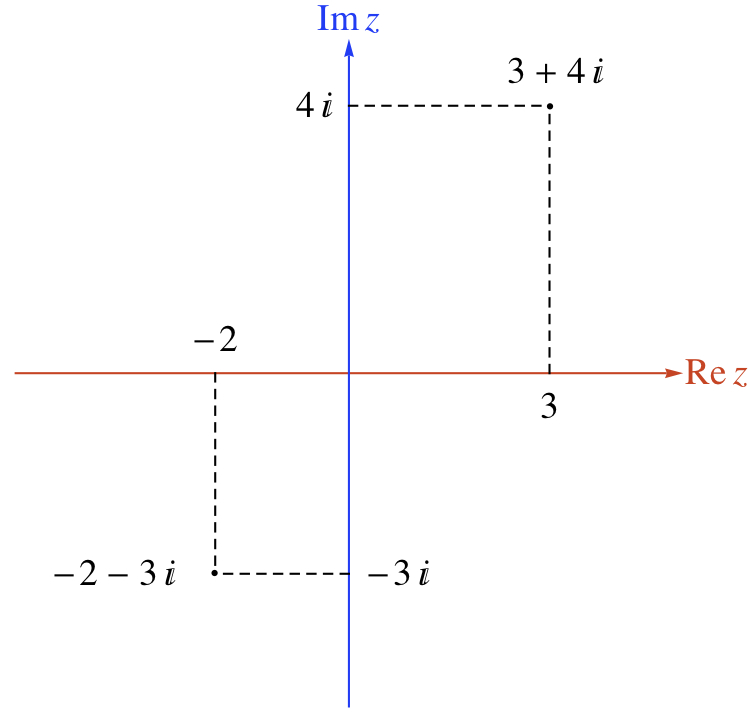
\includegraphics[scale=.6]{img/complexplane.jpg}
\end{center}
Each complex number
is written as $a+b\,i$ with $a$ and $b$ real numbers.  To picture
this, think of $a+b\,i$ as the point $(a,b)$ in the $xy$-plane.
Then $a+b\,i$ is a point in the plane, which in this context
we call the \emph{complex plane}.  The horizontal axis is called
the \emph{real axis} and the vertical axis 
is called the \emph{imaginary axis}.

Addition of two complex numbers is the same as the addition of
two vectors in the plane.  The negation of a complex number is
just the negation of the corresponding vector.  Multiplication
by real numbers is just scalar multiplication, but multiplication
by complex numbers is a combination of rotation and scaling
(try it out!).

Complex conjugation is just the reflection of the vector through the real
axis.  So if $z = a+b\,i$ then $\overline{z} = a-b\,i$.  

The modulus of $z$ is just the length of the vector representing $z$.
(Recall that the length of the vector from the origin to $(a,b)$ is
$\sqrt{a^2+b^2}$. )

\section{Polar Form of Complex Numbers} 



These are also called ``polar coordinates'' and show up in 
Calculus II, for the real plane.  


 \begin{center}
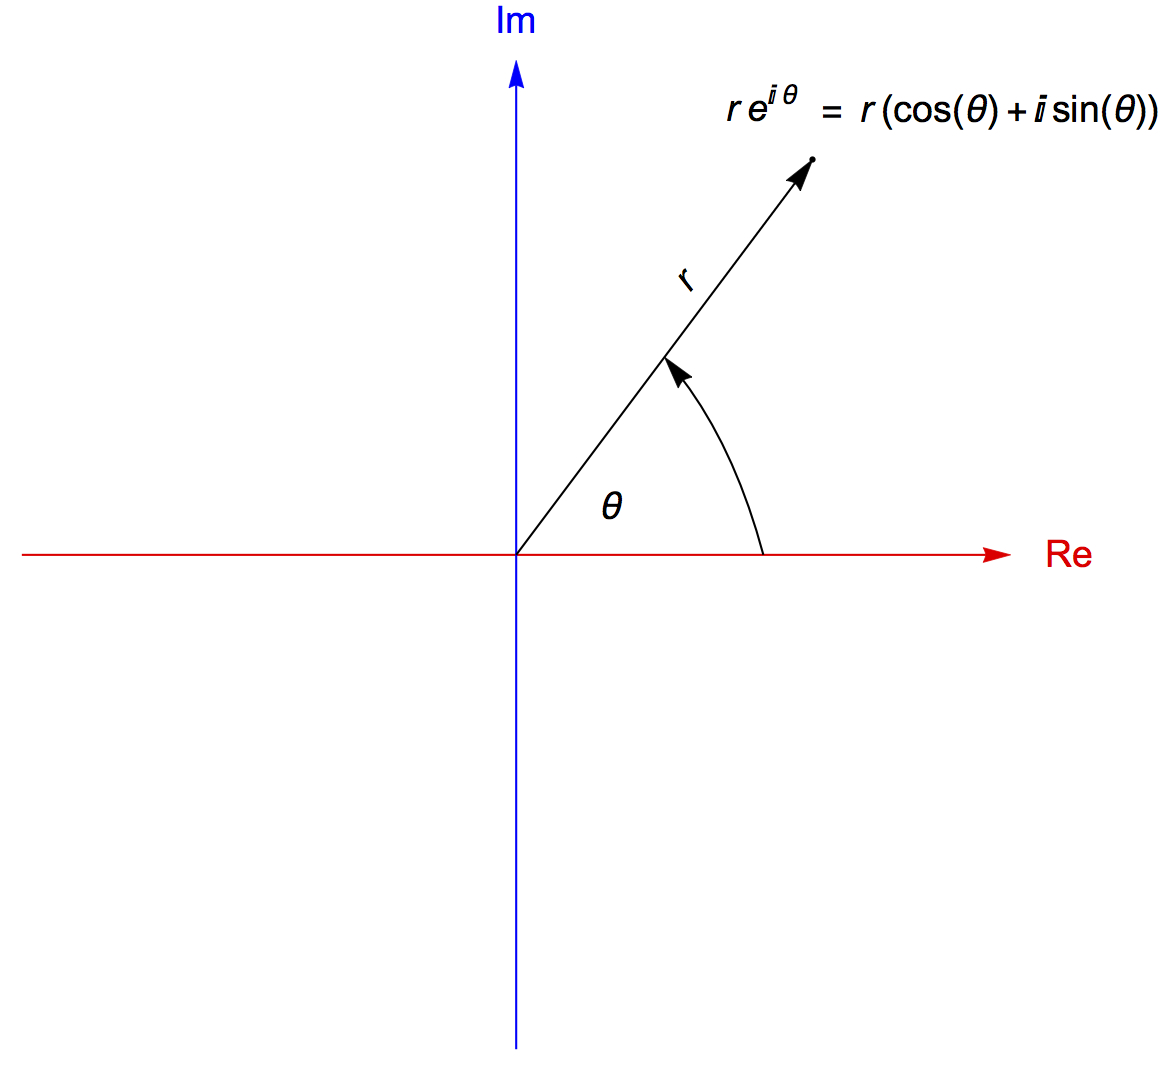
\includegraphics[scale=.5]{img/PolarForm.jpg}
\end{center}




So if $z = x+y\,i \in \C$ then 
$$
\frac{x}{r} = \cos(\theta), \quad \frac{y}{r} = \sin(\theta)
$$
and
$$
r = \vert z \vert = \sqrt{x^2+y^2}
$$
Therefore:  
$$
z = x+yi = r \cos(\theta) + i r\sin(\theta) = r(\cos(\theta)+i \sin(\theta)).
$$
(Note that $\theta = \arg(z)$ (argument of $z$) is not uniquely determined,
since $\theta' = \theta + 2n\pi$, $n\in \Z$, also works.  We usually
pick $-\pi < \theta \leq \pi$ and write $\theta = \Arg(z)$, the principal
argument of $z$.)

In 1748, Euler proved
$$
e^z = 1 + z + \frac{z^2}{2} + \cdots = \sum_{n=0}^\infty \frac{z^n}{n!}
$$
(power series) so in fact by comparing power series with trig functions
we get, surprisingly,
$$
e^{i\theta} = \cos(\theta) + i\sin(\theta).
$$ 
So modern notation is:  the \emph{polar form} of the complex number $z$
is 
$$
z = r e^{i\theta}.
$$

\begin{example}
See the diagram below and check that  $2i= 2e^{i \frac{\pi}2}$, $-i=e^{-i \frac{\pi}2}$, $-1 = e^{i\pi}$, and  
$1+i =\sqrt{2}e^{i \frac{\pi}4}$
\end{example}
\begin{center}
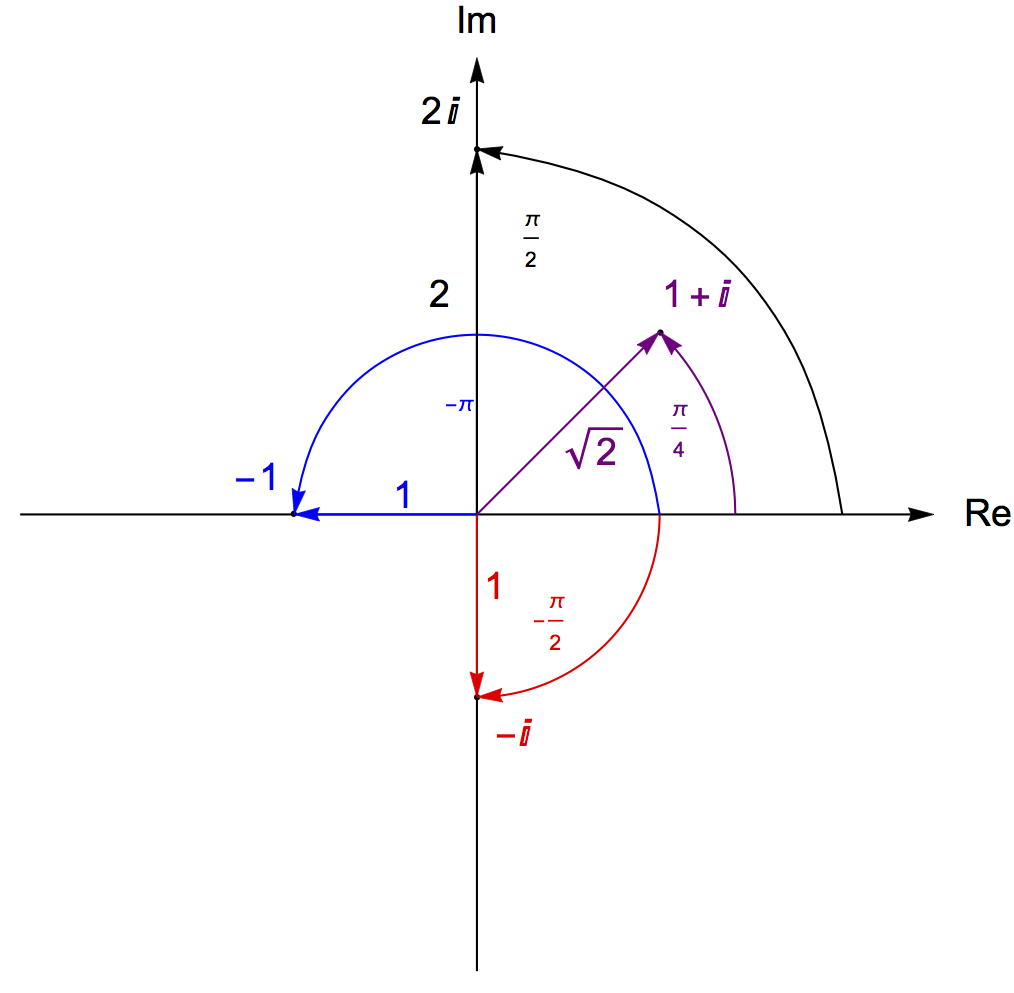
\includegraphics[scale=.6]{img/PolarFormExample.jpg}
\end{center}


We have
\begin{itemize}
\item  $re^{i\theta} = r' e^{i\theta'}$ iff $r=r'$ and $\theta = \theta' + 2n\pi$, some $n\in Z$.
\item $\overline{re^{i\theta}} = re^{-i\theta}$
\item $\vert e^{i\theta} \vert = 1$ for any $\theta$
\end{itemize}

\section{Multiplying complex numbers in polar form}

Note that if $z = re^{i\theta}$ and $w = se^{i\phi}$ then
\begin{align*}
zw &= \left( r(\cos(\theta)+i\sin(\theta)) \right) \left(s (\cos(\phi)+i\sin(\phi)\right) \\
&= (rs)\left( (\cos(\theta)\cos(\phi) - \sin(\theta)\sin(\phi)) + i(\cos(\theta)\sin(\phi) + \sin(\theta)\cos(\phi)) \right)\\
&= rs(\cos(\theta + \phi) + i\sin(\theta + \phi))\\
&= rse^{i(\theta+\phi)}
\end{align*}
That is:  it's like the usual multiplication with exponents.  (Same for
division.)
 
\begin{myprob}
Compute
$$
\frac{i}{1+i}
$$

\begin{mysol}
From before, we have $i = e^{i\frac{\pi}{2}}$ and 
$1+i = \sqrt{2}e^{i\frac{\pi}{4}}$
so
$$
\frac{i}{1+i} = \frac{e^{i\frac{\pi}{2}}}{\sqrt{2}e^{i\frac{\pi}{4}}}
 = \frac{1}{\sqrt{2}}e^{i\frac{\pi}{4}}
$$
(check, using the long method!)

\end{mysol}
\end{myprob}

\section{The Fundamental Theorem of Algebra}



We noted above that every quadratic polynomial with real
coefficients has two roots, and in fact if one root was
complex and not real, then so was the other, and the two
roots are complex conjugates.

Conversely, given a complex number $z$, one polynomial
with roots $z$ and $\overline{z}$ is 
$$
(x-z)(x-\overline{z}) = x^2 -(z+\overline{z})x + z \overline{z}.
$$
Is this a polynomial with real coefficients?  YES!  Write
$z = a+ib$, then $z+\overline{z} = 2a$, which is real; and
$z \overline{z}$ is real (as we proved earlier).  

So:  every real polynomial has complex roots, and every
complex number is the root of some real polynomial.  

That said, if you take two complex numbers $z$ and $w$ which
are not conjugate, then $(x-z)(x-w)$ will just be some
random quadratic polynomial with complex coefficients.
Which begs the question:  if you take all quadratic polynomials
with complex coefficients, and use the quadratic formula to
solve them, what extra numbers (like $i$) do you need this 
time?  

Answer:  NONE.  The complex numbers are the top of the heap,
and all you'll ever need:

\begin{theorem}[Fundamental Theorem of Algebra]
Every polynomial with coefficients in the complex numbers
factors completely into linear factors of the form $ax+b$,
with $a,b \in \mathbb{C}$.
\end{theorem}

\section[Some musings about the Fundamental Theorem of Algebra]{Some musings about the meaning of the Fundamental
Theorem of Algebra}

 This answers a really big nagging problem
of algebra: shouldn't every quadratic have 2 roots, and 
every cubic 3 (allowing multiple roots)?  But the quadratic
$x^2+2$ didn't have any roots over the reals.  

In Calculus,
we accept this by sketching the graph of $y=x^2+2$ and saying,
``Look, it doesn't intersect the $x$-axis.  That explains it.''

``Explains what, exactly?'' an algebraist responds.  ``You're 
still missing two roots.''  

In algebra, we are looking for unifying themes, things that
are common across all problems of a particular type.  We look
for wonderful universal solutions.  The complex numbers are
one example of a universal solution:  we added $\sqrt{-1}$
and suddenly all problems were solved:  $x^2+2$ has two roots,
and $ix^7+3x^2-(4+i)$ has 7 roots.  

(Well, one might admit, not all problems are completely solved.
The Fundamental Theorem of Algebra doesn't say ANYTHING about
FINDING the roots.  It just says that they exist.  We end up
going back to Calculus for help in finding them.)

For the rest of this course, we will be considering LINEAR algebra,
which is a particular branch of algebra where, it turns out, there
are fantastically universal solutions to absolutely everything
(not just ``existence'', but actually ways of finding solutions!).


%
% Use the following environment.
% Don't forget to label each problem;
% the label is needed for the solutions' environment
